\documentclass[11pt,twocolumn]{article}
\bibliographystyle{siam}

\usepackage[margin=0.75in]{geometry}
\usepackage{graphicx}

\title{\textbf{Team Zeta Project Report}\\
Visual Object Prediction by Machine Learning:\\ 
Object Category Approximation Using Non-Maximal Voxels}
\author{
  Chen, Tzu-Chieh\\
  \texttt{tcchenbtx}
  \and
  Ho, Edith\\
  \texttt{edithhcw}
  \and
  Marediya, Zubair\\
  \texttt{zubair-marediya}
  \and
  Tran, Mike\\
  \texttt{miketranx4}
  \and
  Zhang, Dongping\\
  \texttt{dpzhang}
}

\begin{document}
\maketitle

\abstract{}
If we present different categories of 
picture stimulus to a subject, would each stimulus category  evoke the 
same category-specific pattern of response in the ventral object vision 
pathway? Furthermore, can we distinguish individual categories from the 
patterns of response evoked? Using the patterns of response evoked, could
we predict what category the stimulus is?


\section{Introduction}

Haxby et al's study, \emph{Distributed and Overlapping Representations of Faces
and Objects in Ventral Temporal Cortex}\cite{objectrec}, collected data 
from a sample of six subjects of which consists of five females and one male. 
It presented two categories of natural stimuli, which are faces, cats, 
five categories of man-made objects, which are chairs, shoes, bottles, tools, houses, and non-sense pictures of phase-scrambled images, to each subject. 
The study wanted to answer the questions: if we present different categories of 
visual stimuli to a subject, would each visual stimulus category evoke the 
same category-specific pattern of response in the ventral object vision 
pathway? Could we distinguish individual categories from the 
patterns of response evoked? \\

Each subject were placed into the functional 
magnetic resonance imaging (fMRI) for 12 times thus generating 12 time series 
data. One complete experiment run lasted 300s. It began with 12s of rest, followed by 8 stimulus blocks of 24s duration, one for each category of visual stimuli. There were 12s intervals of rest between any two stimulus blocks, and 
the whole procedure ended with another 12s of rest. 
During each stimulus blocks, each picture stimulus were presented for 0.5s 
followed by an interstimulus interval for 1.5 ms, thus presented a total of 
12 stimuli during 
each stimulus block and 96 stimuli in a complete experiment run.\\

In Haxby et al's study, the data collected for each subject were split into two 
runs: odd runs and even runs. Correlation were used as indices of response similarity, and from 
analyzing within-category correlation and between-category correlation, the 
result suggested that category-specific patterns of response were distributed 
and overlapping. The result brought a new question of whether each stimulus 
category evoked a distinct pattern of response in cortex that responded 
maximally to other categories. To test whether the patterns of non-maximal 
responses carry category-related information, voxels that responded maximally 
to either category were excluded from calculation of correlations. It turned 
out that removal of maximally responded voxels from correlation calculation 
barely diminished the accuracy of identification. The research reached a 
conclusion that the pattern of large and small responses, not just the location 
of large responses, carry category-related information, and small responses 
are an integral part of the representation.\\

\section{Data}

The study's curated dataset can be found and downloaded on the OpenfMRI 
database\cite{fmriData} with ds105's accession number. The ds105 
sub-directory contains files detailing this study, including general information 
(README file), related research articles (references.txt), detail information 
and update for this released dataset (release\textunderscore history.txt), 
the MR repetition time (scan\textunderscore key.txt), the name 
(study\textunderscore key.txt), and the major task for this study 
(object viewing) (task\textunderscore key.txt). In addition, the models folder 
contains files with the key conditions (list of object categories) 
(condition\textunderscore key.txt) and the comparison setting in this study 
(tast\textunderscore contrasts.txt). \\

Subjects have individual directories storing their results. There are four 
sub-directories in each of the respective directories. The anatomy 
sub-directory contains high-resolution scans of the subject's head 
(highres001.nii.gz), mask for obtaining the ``brain only'' scans 
(highres001\textunderscore brain\textunderscore mask.nii.gz), and the 
``brain only'' anatomy result (highres001\textunderscore brain.nii.gz). 
The ``behav" sub-directory is empty since subject's behavior is irrelevant 
to this study. The ``model" sub-directory provides information such as the 
onset time (in seconds), and the duration and weighting for each conditions 
(object category) for the 12 task runs in this study. The ``BOLD" sub-directory 
contains fMRI results for all 12 task runs for each subject respectively. 
In each task run directory, we can find the fMRI result (bold.nii.gz) and 
a QA sub-directory with that run's time series analysis report, fMRI results
pre-processing and confound files, and visualization of the brain (nii files).\\ 

\section{Methods}

Within each subject, for each of the twelve runs, we have eight condition
files corresponding to each of the eight objects in our study. Each
condition file consists of time points of when the corresponding object 
showed up in the run. We run the event2neural() function on this condition
file, and it returns an array of 121 values of zero or one. These indicate
time intervals at which the subject was looking at that particular object.
We then used the convolve function within numpy to convolve the bold signal
for this object onto all the specified time intervals. After repeating this
for each object, we were able to create regressors and build our design
matrix. Lastly, we fit a linear model to the predicted BOLD signal we got
from convolution, and gathered a mean RSS value. We then applied the contrast
function to see whether a particular object showed a pattern in the brain.
Unfortunately, the voxels gave off images that were too defined, making it hard
to see any patterns. Thus, we applied a Gaussian filter to smooth over the
values and blur the images. This led to us seeing patterns a bit better.
This is explained below. \\

With the rest of the unprocessed data, what we plan to do is to repeat our
cleaning data process. This involves removing outliers in the intensity data,
smoothing the voxel data, and reducing the dimensionality of the data. In
terms of smoothing the data, the following steps were taken to do so:
First, grab all the voxel intensity values and store it in an array.
Then, iterate through each voxel intensity value, then apply Gaussian filter
to that point. This produces a smooth voxel while increasing the blur, which
makes it easier to see patterns or trends in the brain. This method is
appealing to the human eye, however the caveat is that the new patterns
a person might see could actually be false signals since the data was
transformed. Finally, the method we are considering to make use of for
dimension reduction is Principal Component Analysis (PCA). PCA will
essentially extract features from the original data, control variance in the
data, and convey more information with less dimensions. Finally, in order to
validate our models and data analysis, we'll be looking at mean square error
and classification rate as metrics to judge how well our model performs. \\

In terms of what statistical methods we will employ on the data, below is a
general description of the statistical method and its purpose, specifically�
with our data. Generalized linear models can be utilized to build other linear
models off the data, with different assumptions behind the data. For example,
we could assume the error distribution models something other than a normal
distribution. ANOVA tests if different groups have the same mean, while
Kruskal-Wallis Test tests the hypothesis of whether or not each group�
comes from the same distribution. This will be applied to see if the fMRI data
of different objects are statistically significant. One other subject that
would be interesting to look at is time series analysis. The BOLD signals�
constitute time series data; thus, some methods that can be used include
forecasting, ARIMA or GARCH fitting, and specifying P, D, and Q. Finally,
one investigation we are going to look into is to determine whether or not
the BOLD signals are normally distributed. \\

Some other analysis we could consider, given time, would be to try using
machine learning to see if we can build models that can predict objects seen
by the subject. Some models that could solve this problem include random
forests and boosting. Until then, our main focus will be on the previous
statistical methods we described earlier. \\

\section{Results}

After downloading the data from open fMRI database, the data for 
sub001 run001 was used to perform initial analysis to see if we can identify 
specific brain region for recognizing specific object like house. 

First, functions from homework 2 were used to identify outliers and remove 
them. 
\begin{figure}[h!]
\centering
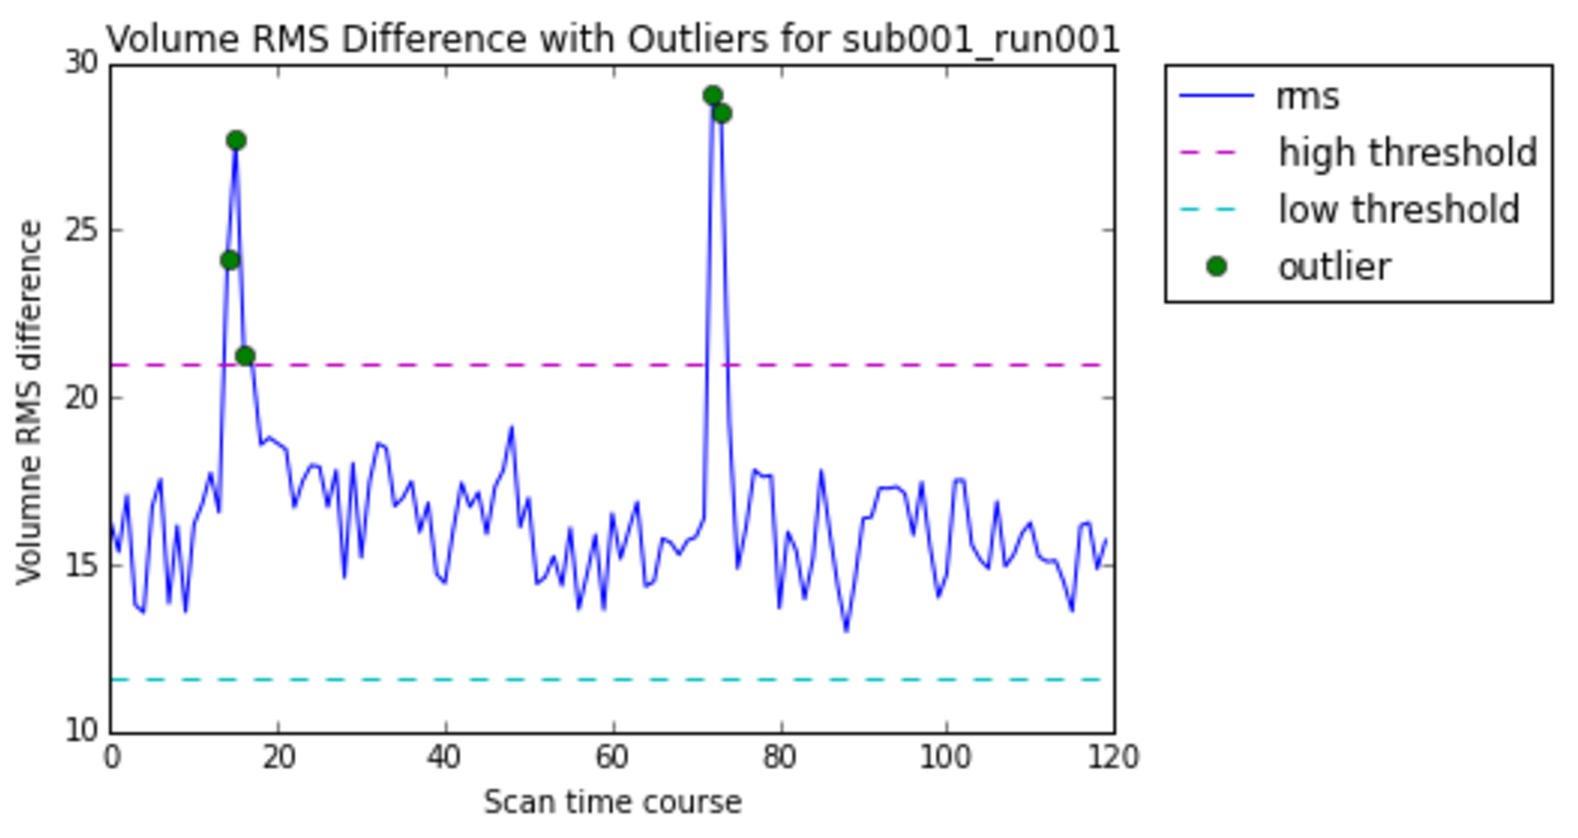
\includegraphics[width=120mm]{outlier.png}
\caption{Outliers}
\end{figure}

Secondly, we used envents2neural function to generate task time course. 
\begin{figure}[h!]
\centering
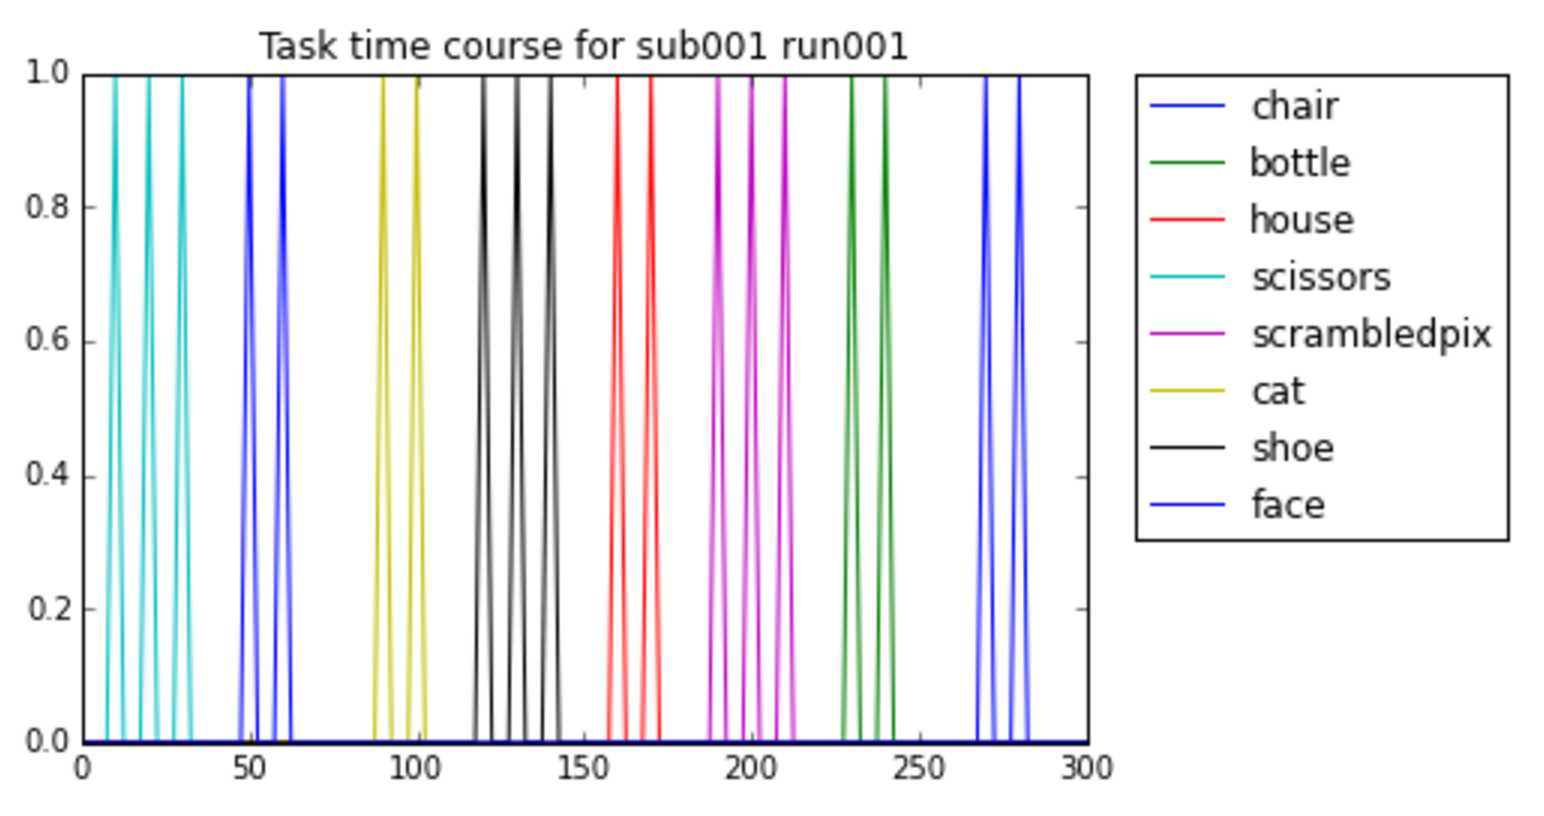
\includegraphics[width=120mm]{task_time_course.png}
\caption{Task Time Course}
\end{figure}

\pagebreak 

Thirdly, we performed convolusion to generate predicted BOLD signals for this 
dataset.
\begin{figure}[h!]
\centering
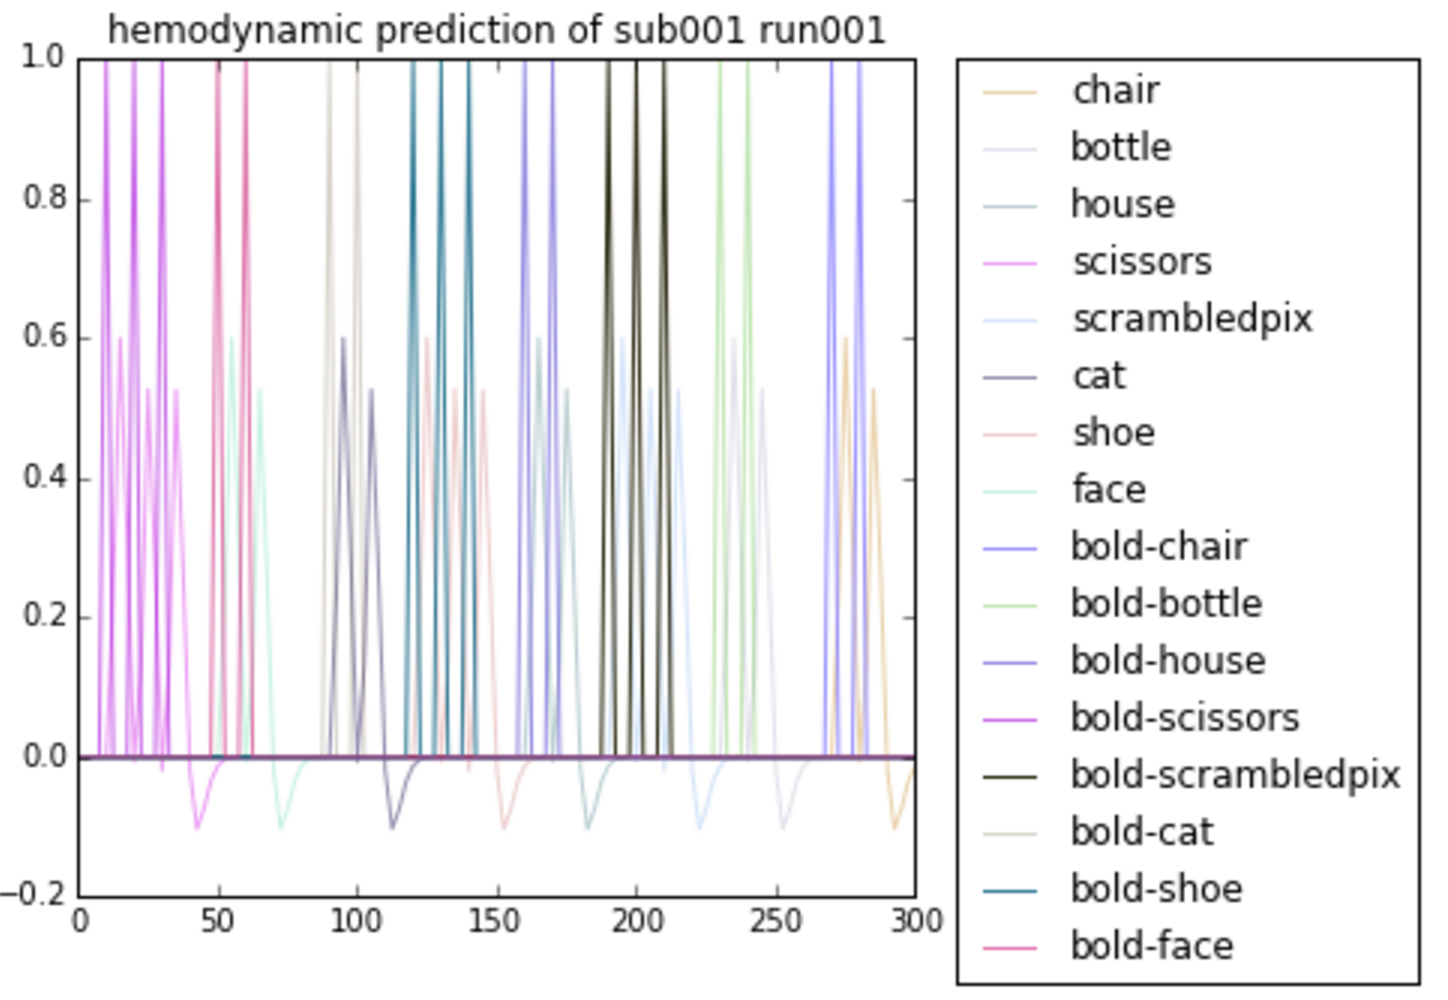
\includegraphics[width=120mm]{stimulation_bold.png}
\caption{Stimulation Bold}
\end{figure}

Finally, these convolved results for each objects were used as parameters in 
our design matrix for linear regression. To avoid the drifting problem, we also 
included two drift parameters in the design matrix. The final design matrix was 
arranged as followed: bottle, cat, chair, face, house, scissors, scrambledpix, 
shoe, drift1, drift2, average(all ones)
\begin{figure}[h!]
\centering
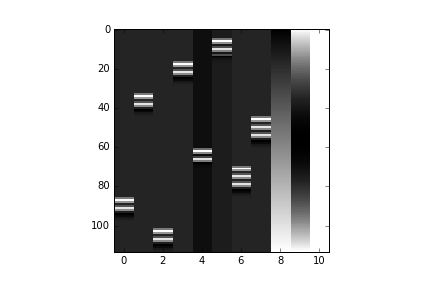
\includegraphics[width=120mm]{design_matrix.png}
\caption{Design Matrix}
\end{figure}

\section{Discussion}

There are a lot of problems that came up during our analysis. To begin with, 
since most of us have limited neuroscience knowledge, it was very difficult to 
merely understand the study and the data itself. The research paper of the 
study uses specific and technical terms that make it hard to comprehend. 
More time was spent at the earlier stages of this project rereading the 
original paper and exploring the data folders than expected, which slowed down 
our progress for analysis. Therefore, we only had time to investigate one 
subject and one run so far. Now that we have a better understanding of the 
study and the data, we hope to repeat our analysis on the remaining subjects.\\

After we understood which part of the data to use, we started our 
exploratory data analysis. There is a lot of noise within the original dataset, 
causing insignificant p-values for test statistics, such as t-tests. Moreover, 
the noise in the original dataset produces low-resolution brain images, 
which are not meaningful for our further analysis. Pre-processing of data, 
including the removal of outliers using techniques from homework 2, was 
performed. In addition, we used smoothing techniques to create clearer 
and more meaningful images. \\

Furthermore, we faced problems recently that are yet to be resolved. Since 
subjects? heads often slowly move to a certain direction during fMRI scans, 
drifting of time series graph of BOLD signals is observed. We are planning 
to apply time series analysis modeling techniques, which will hopefully take 
the drifting into account and improve the accuracy of our models. Also, the 
BOLD signals change differs from subject to subject, making it difficult to 
compare signals from the same run between subjects. We would need to 
find a statistical valid way to standardize the BOLD signals, so we could 
analyze how BOLD signals under different conditions are related to each 
other across subjects. \\

\bibliography{project}

\end{document}
